\newpage
\section{Ablauf}\label{sec:ablauf}
Zur Untersuchung der Kommunikation zwischen der Geräten wird der Verkehr auf den
(W)LAN-Schnittstellen in verschiedenen Szenarien betrachtet:

\begin{enumerate}
    \setlength\itemsep{-0.5em}
    \item Jeweils eine Minute ohne Aktionen bei ein- und ausgeschalteter Konsole
    \item Ein- und Ausschalten über \textit{Hassbian}
    \item Ein- und Ausschalten über \textit{Harmony Hub}
\end{enumerate}

Da alle in den Szenarien betrachteten Verbindungen LAN-Verbindungen sind,
werden die entsprechenden Pakete über den zentralen Router des lokalen Netzwerks transportiert.
Folglich ist dies auch ein passender Punkt um den auftretenden Verkehr mitzuschneiden.
Bei dem Router handelt es sich um eine \textit{FRITZ!Box 7560} \cite{FRITZBox29:online}.
Wie auch andere FRITZ!Boxen stellt diese unter der Adresse \nolinkurl{http://fritz.box/html/capture.html} eine Oberfläche bereit,
um Datenpakete an verschiedenen Schnittstellen mitzuschneiden und diese Paketmitschnitte
in einem für das bekannte Tool \textit{Wireshark} lesbaren Format herunterzuladen.

\begin{figure}[ht!]
    \centering
    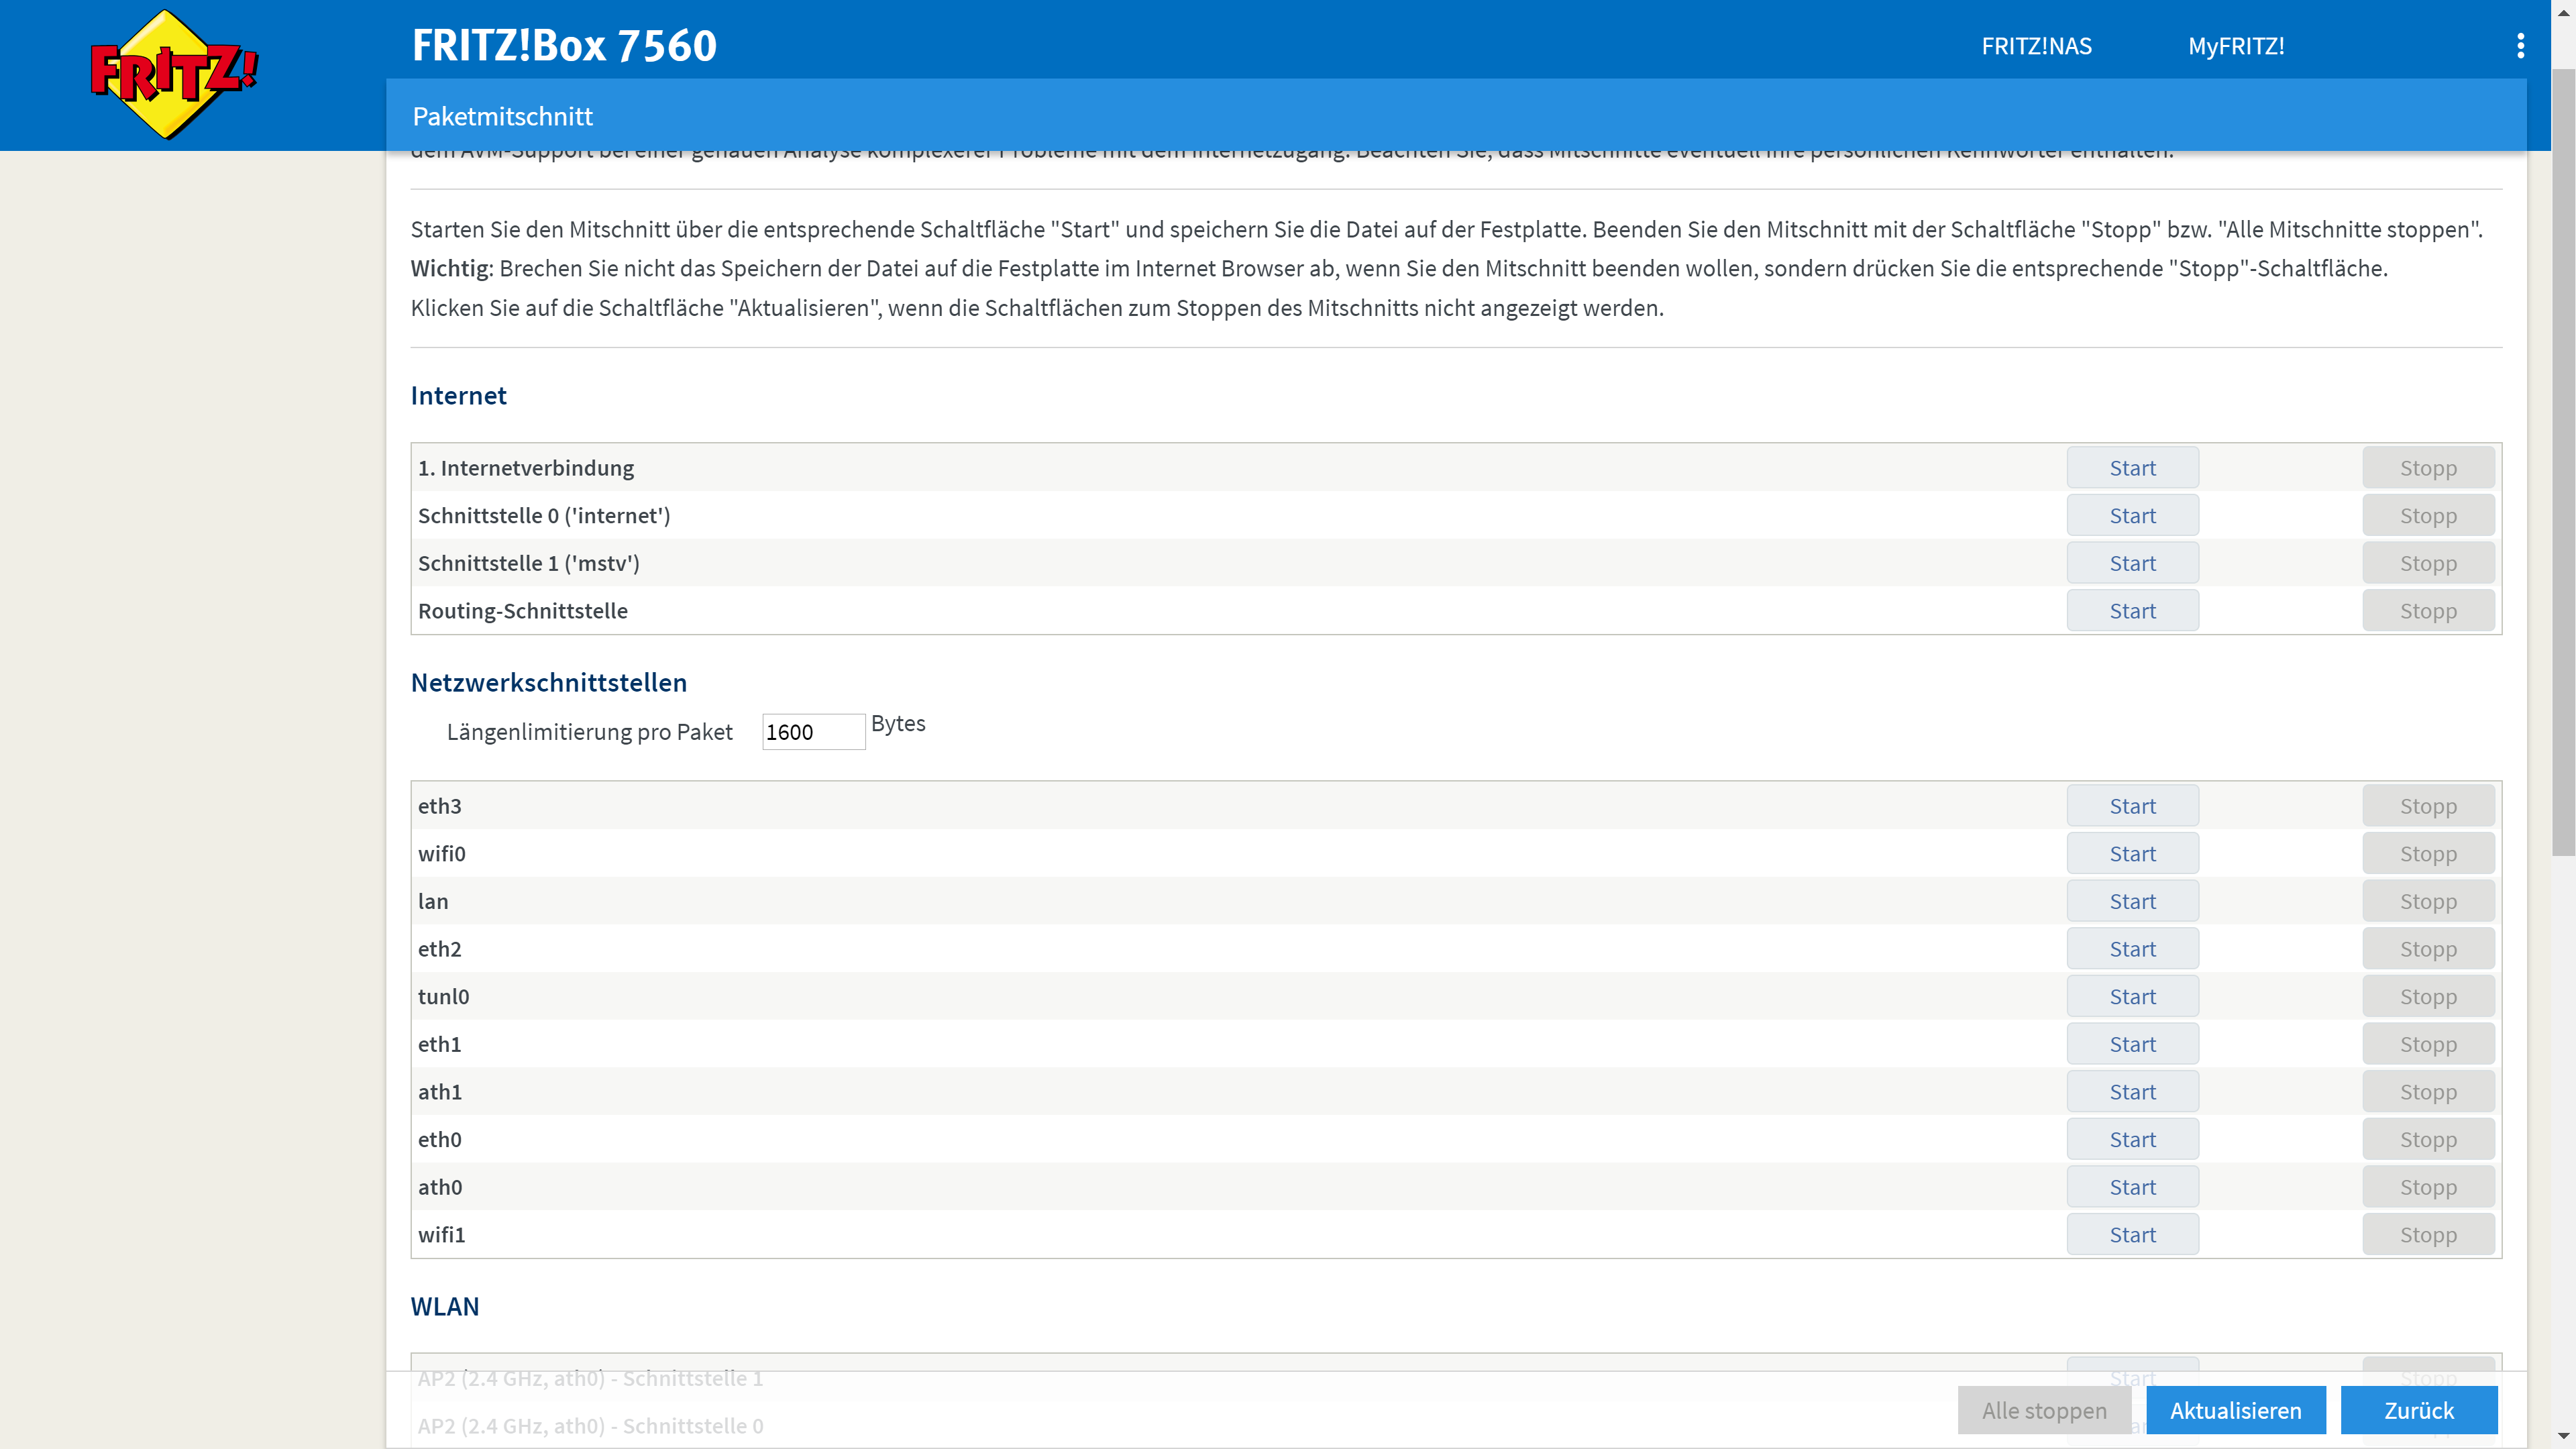
\includegraphics[width=0.75\textwidth]{fribCapture}
    \caption{FRITZ!Box Weboberfläche für Paketmitschnitte}\label{fig:fribCapture}
\end{figure}

Diese Methode bringt zwei Vorteile mit sich:
Zum einen läuft der gesamte Verkehr durch den Router, da alle Geräte per (W)LAN an diesen angeschlossen sind.
Zum anderen können dort die Pakete unkompliziert mitgeschnitten werden. Zugriff auf die zu betrachtenden Geräte
oder gar ein Umleiten des Verkehrs auf einen Computer, beispielsweise durch \textit{Spoofing} \cite{Maninthe12:online} sind nicht notwendig.

Jedoch hat diese Methode auch einen Nachteil:
Die Oberfläche für Paketmitschnitte ist nicht für den allgemeinen Nutzer bestimmt.
Eigentlich dient sie nur zur Unterstützung des Supports bei komplexen Problemen.
Daher wird die Funktion auch nicht offzizell dokumentiert.
Lediglich eine kurze Anleitung wie solle Paketmitschnitte gestartet und gestoppt werden befindet sich im oberen Bereich der Seite.
Die zahlreichen Schnittstellen (wie \texttt{Routing}, \texttt{lan}, \texttt{ath0}, \texttt{ath1}, \texttt{eth0}, ...) werden nicht näher spezifiziert.

Hinweise auf den Zweck der verschiedenen Schnittstellen liefert zum Beispiel Jeroen Wiert Pluimers.
In \cite{fritzcap8:online} präsentiert er seine Ergebnisse einer Analyse der Schnittstellen.
Hier hervorzuheben ist die Schnittstelle \texttt{ath0}.
Als WLAN-Schnittstelle scheint sie gut für dieses Projekt geeignet zu sein.

Ein praktischer Vergleich mit den Schnittstellen \texttt{lan} und \texttt{Routing} zeigt,
dass in dem Mitschnitt von \texttt{ath0} alle Pakete der zu betrachtenden Komponenten enthalten sind.

Der Mitschnitt von \texttt{lan} enthält zwar auch alle Pakete der zu betrachtenden Komponenten.
Er enthält jedoch auch viele andere Pakete, was die Übersicht über die auftretenden Pakete stark beeinrächtigt.

Der Mitschnitt der \texttt{Routing}-Schnittstelle enthält lediglich Pakete welche vom Router an das Internet gesendet
oder aus diesem empfangen werden.
Diese Schnittstelle ist daher für den lokalen Verkehr ungeeignet.

Das Erfassen der Pakete die Szenarien geschieht nach folgendem Muster:
\begin{enumerate}
    \setlength\itemsep{-0.5em}
    \item Starten des Paketmittschnitts auf \texttt{ath0}
    \item Durchführen des Szenarios
    \item Beenden des Paketmittschnitts
    \item Öffnen des Mitschnitts mit \textit{Wireshark} und Filtern der relevanten Pakete
    \item Speichern des gefilterten Mitschnitts zur späteren Analyse
\end{enumerate}